%Version 3.1 December 2024
% See section 11 of the User Manual for version history
%
%%%%%%%%%%%%%%%%%%%%%%%%%%%%%%%%%%%%%%%%%%%%%%%%%%%%%%%%%%%%%%%%%%%%%%
%%                                                                 %%
%% Please do not use \input{...} to include other tex files.       %%
%% Submit your LaTeX manuscript as one .tex document.              %%
%%                                                                 %%
%% All additional figures and files should be attached             %%
%% separately and not embedded in the \TeX\ document itself.       %%
%%                                                                 %%
%%%%%%%%%%%%%%%%%%%%%%%%%%%%%%%%%%%%%%%%%%%%%%%%%%%%%%%%%%%%%%%%%%%%%

%%\documentclass[referee,sn-basic]{sn-jnl}% referee option is meant for double line spacing

%%=======================================================%%
%% to print line numbers in the margin use lineno option %%
%%=======================================================%%

%%\documentclass[lineno,pdflatex,sn-basic]{sn-jnl}% Basic Springer Nature Reference Style/Chemistry Reference Style

%%=========================================================================================%%
%% the documentclass is set to pdflatex as default. You can delete it if not appropriate.  %%
%%=========================================================================================%%

\documentclass[sn-basic]{sn-jnl}% Basic Springer Nature Reference Style/Chemistry Reference Style
\setcitestyle{numbers} 
%\documentclass[pdflatex,sn-basic]{sn-jnl} 


\usepackage{graphicx}%
\usepackage{multirow}%
\usepackage{amsmath,amssymb,amsfonts}%
\usepackage{amsthm}%
\usepackage{mathrsfs}%
\usepackage[title]{appendix}%
\usepackage{xcolor}%
\usepackage{textcomp}%
\usepackage{manyfoot}%
\usepackage{booktabs}%
\usepackage{algorithm}%
\usepackage{algorithmicx}%
\usepackage{algpseudocode}%
\usepackage{listings}%
%%%%





\raggedbottom
%%\unnumbered% uncomment this for unnumbered level heads

\begin{document}

\title[Modelling of scenario discovery]{Modelling of the modelling process. }
\subtitle{A Scenario Discovery case study}
%%=============================================================%%
%% GivenName	-> \fnm{Joergen W.}
%% Particle	-> \spfx{van der} -> surname prefix
%% FamilyName	-> \sur{Ploeg}
%% Suffix	-> \sfx{IV}
%% \author*[1,2]{\fnm{Joergen W.} \spfx{van der} \sur{Ploeg} 
%%  \sfx{IV}}\email{iauthor@gmail.com}
%%=============================================================%%

\author*[1]{\fnm{Giulia} \sur{Vannucci}}\email{giulia.vannucci@unina.it}

\author[2,3]{\fnm{Samuele} \sur{Lo Piano}}\email{samuele.lo.piano@pg.edu.pl}
%\equalcont{These authors contributed equally to this work.}

\author[4]{\fnm{Anald} \sur{Puy}}\email{a.puy@bham.ac.uk}
%\equalcont{These authors contributed equally to this work.}

\author[1]{\fnm{Roberta} \sur{Siciliano}}\email{roberta@unina.it}
%\equalcont{These authors contributed equally to this work.}

\author[5,3]{\fnm{Andrea} \sur{Saltelli}}\email{andrea.saltelli@uib.no}
%\equalcont{These authors contributed equally to this work.}



\affil*[1]{\orgdiv{Department of Electrical Engineering and Information Technology}, \orgname{University of Naples Federico II}, \orgaddress{\street{Via Claudio, 21}, \city{Naples}, \postcode{80125},  \country{Italy}}}

\affil[2]{\orgdiv{Faculty of Management and Economics}, \orgname{Gdańsk University of Technology}, \orgaddress{\street{G. Narutowicza Street 11/12}, \city{Gdańsk}, \postcode{80233}, \country{Poland}}}

\affil[3]{\orgdiv{Barcelona School of Management}, \orgname{Universitat Pompeu Fabra}, \orgaddress{\street{Carrer de Balmes 132}, \city{Barcelona}, \postcode{08008},  \country{Spain}}}

\affil[4]{\orgdiv{School of Geography, Earth and Environmental Sciences}, \orgname{University of Birmingham}, \orgaddress{\street{Edgbaston }, \city{Birmingham}, \postcode{B15 2TT},  \country{United Kingdom}}}

\affil[5]{\orgdiv{Centre for the Study of the Sciences and the Humanities}, \orgname{University of Bergen}, \orgaddress{\street{Parkveien 9} \city{Bergen}, \postcode{PB 7805, 5020},  \country{Norway}}}


\abstract{Abstract}


\keywords{keyword1, Keyword2, Keyword3, Keyword4}

%%\pacs[JEL Classification]{D8, H51}

%%\pacs[MSC Classification]{35A01, 65L10, 65L12, 65L20, 65L70}

\maketitle


\section{Introduction}

In the present work we investigate scenario discovery, an activity of exploratory modelling analysis and machine
learning applied to the output of Integrated Assessment Models (IAMs). 



\textcolor{red}{%
The method answers a real difficulty: IPCC-class ensembles run to thousands of
pathways, too many to read one by one, and scenario discovery promises to mine
them for structure --- partitioning the space of assumptions into regions that
do or do not reach a target and ranking the input factors by their apparent
influence. A typical pipeline chains a classifier (e.g.\ a random forest) to a
feature-importance step (permutation importance or SHAP) and a rule-extraction
method such as PRIM, yielding compact ``if--then'' boxes and ordered lists of
decarbonisation ``drivers''. The promise is that pooling many scenarios and
analysing them collectively yields the ``robust insights'' no single scenario
can offer
\citep{Guivarch_Le_Gallic_Bauer_Fragkos_Huppmann_Jaxa-Rozen_Keppo_Kriegler_Krisztin_Marangoni_et_al._2022};
the method is now taught in its own right, as at the 2026 PRISMA summer school
\citep{university_of_geneva_prisma_2026}.}

\textcolor{red}{%
A ranking of drivers extracted from an ensemble, however, is a property of two
things at once: the system the models represent, and the ensemble the analysts
built --- its sampled dimensions, its classifier, its importance metric, its
success threshold. Which of the two dominates is an empirical question, and it
is the one we address here.}


We move from the AR6 database
\citep{Byers_Krey_Kriegler_Riahi_Schaeffer_Kikstra_Lamboll_Nicholls_Sandstad_Smith_et_al._2022}
$\approx 1,200$ vetted scenarios in the IIASA explorer
\citep{Kikstra_Nicholls_Smith_Lewis_Lamboll_Byers_Sandstad_Meinshausen_Gidden_Rogelj_et_al._2022}.

We take a documented,
fully public scenario-discovery pipeline; treat the analyst's choices as the
input factors --- classifier, feature-importance metric (permutation vs.\
SHAP), temperature-binning, PRIM peeling and coverage thresholds; treat the
discovered driver-ranking as the output; and run a global sensitivity analysis
on that map. 




Our analysis is called elsewhere Modelling of the Modelling Process (MOMP)  \citep{saltelli_mathematical_2024, saltelli_what_2023,
lachi_robustification_2025}, and continues a series of works where a combination of sensitivity analysis and uncertainty quantification is used to criticize the practice of IAMs \citep{saltelli_sensitivity_2010}, and that of ambitious modelling of the planet \cite{saltelli_bring_2024, Saltelli_Melsen_Puy_2025}. The critique is part of a more general call for responsible modelling \citep{saltelli_five_2020,  Saltelli_Di_Fiore_2023,
saltelli_equations_2026}. 

Similar criticism is found in water resources and hydrology --- where the ``delusive accuracy'' of a widely used global estimate is documented \cite{Puy_Sheikholeslami_Gupta_Hall_Lankford_Lo_Piano_Meier_Pappenberger_Porporato_Vico_et_al._2022} --- and on energy \cite{lo_piano_energy_2025}.

\textcolor{red}{[To include, possibly]. Arnald and co-workers have a paper in progress applying a
similar deconstruction to GRACE and GRACE-FO, the main instrument behind the
global water-crisis narrative.}

The work \cite{Puy_Beneventano_Levin_Lo_Piano_Portaluri_Saltelli_2022} further anatomises problem with some of these modelling  studies by showing that higher effective dimensionality inflates uncertainty ---
an ensemble whose variance is genuinely high-dimensional cannot carry the
low-dimensional causal story of a few tidy ``drivers.''


In summary, scenario discovery would appear to discover the
analyst, rather than the future. 


\section{Previous works}

The work \cite{Jaxa-Rozen_Trutnevyte_2021} already finds that a large share of
the spread across 1,550 scenarios traces to general features --- the type of
organisation, the model, broad policy assumptions --- rather than to specific
techno-economic inputs, with IPCC scenarios systematically projecting lower
photovoltaic uptake. They used XGBoost with SHAP values (their Fig.~6) and
topic-modelling to attribute the variance. A result showing that ``which
institution ran it'' predicts the outcome better than the physical-economic
parameters is, read correctly, a finding that the ensemble is an ensemble of
opinion, not of evidence --- though they frame it as a call
for ``more organisational diversity in IPCC scenario design.'' Their SHAP
feature-importance is also squarely within our competence and interest.

\bigskip

The work
\cite{Guivarch_Le_Gallic_Bauer_Fragkos_Huppmann_Jaxa-Rozen_Keppo_Kriegler_Krisztin_Marangoni_et_al._2022}
is a Perspective, not an empirical study --- a programmatic statement by
seventeen authors involved in IAM scenario work. They argue that analysing
scenario ensembles can bring new and more robust insights than single
scenarios, and lay out a three-step approach: (1)~pre-processing the ensemble;
(2)~selecting a few scenarios or analysing the full ensemble; and
(3)~providing users with efficient access to the information. Step~2 is where
scenario discovery, clustering, and the ML feature-attribution methods are
described. The entire framing is robustness --- ``robust insights'' is in the
title, the abstract, and the closing line --- the explicit claim being that
pooling many scenarios manufactures robustness that single scenarios lack. It
has no empirical pipeline to reproduce, but it is the doctrine.
We can therefore cite it as the doctrine --- ``the community
holds that large ensembles yield robust insights'' --- and then hold up the
instances below against it, running the GSA-on-the-procedure demonstration on
the public AR6 ensemble to show that the robustness is an artefact of analyst
choice.


\bigskip

Three papers are relevant to our analysis:

\begin{itemize}
     
\item \cite{Lamontagne_Reed_Link_Calvin_Clarke_Edmonds_2018} is the
natural point of origin: it adopts the exploratory-modelling school and may be
the actual origin of decision-relevant scenario discovery applied to GCAM
climate-economic ensembles --- a statement of the method applied to
decarbonisation futures.

\item \cite{Li_Pye_Keppo_Jaxa-Rozen_Trutnevyte_2023} is one study taken as target of the present analysis. It claims to ``reveal robust insights into regional decarbonisation
strategies'' using exactly the RF~$\rightarrow$~logistic-regression~$\rightarrow$~PRIM
pipeline the PRISMA school teaches, on the public IPCC SR1.5 database, and it
makes strong, concrete policy claims (decommission unabated gas, prioritise
solar and electrification, bioenergy pivotal in Latin America). It exemplifies
the ``drivers read off an ensemble'' genre and is fully reproducible (open
access, public database, scikit-learn~$+$~EMA~Workbench, code documented).
\item \cite{Wessel_Iyer_Wild_Ou_McJeon_Lamontagne_2024} is a further
exemplar: it applies scenario discovery to a large GCAM ensemble, sampling
deep uncertainties (technology costs and efficiencies, electrification,
institutional factors, NDCs) to connect ``critical drivers'' to
energy-transition outcomes, with a regional framing on Latin America.


\item \cite{Chiani_Borgonovo_Plischke_Tavoni_2025} uses optimal-transport methods (based on Wasserstein-type distances)
that permit
sensitivity analysis when the output is multivariate. It handles
correlated inputs and can be estimated directly from an input--output dataset
without a special sampling design. \cite{Chiani_Borgonovo_Plischke_Tavoni_2025} apply it to RICE50+ emissions pathways
with up-to-date demographic and socioeconomic input distributions, and report,
for instance, that in the Paris Agreement scenario the main driver is climate
sensitivity followed by carbon intensity, with input importance shifting
across regions and over time. Crucially, this is a GSA of the
\emph{model}, not of the discovery \emph{procedure}. 
\cite{Chiani_Borgonovo_Plischke_Tavoni_2025} applies GSA to IAM outputs to rank physical drivers
in this work instead, we apply GSA to the
scenario-discovery procedure itself, treating the analyst's choices as factors
and the discovered drivers as output.

\end{itemize}



\section{Preliminary results (Arnald on Li et al.)}
\begin{figure}[htbp]
    \centering   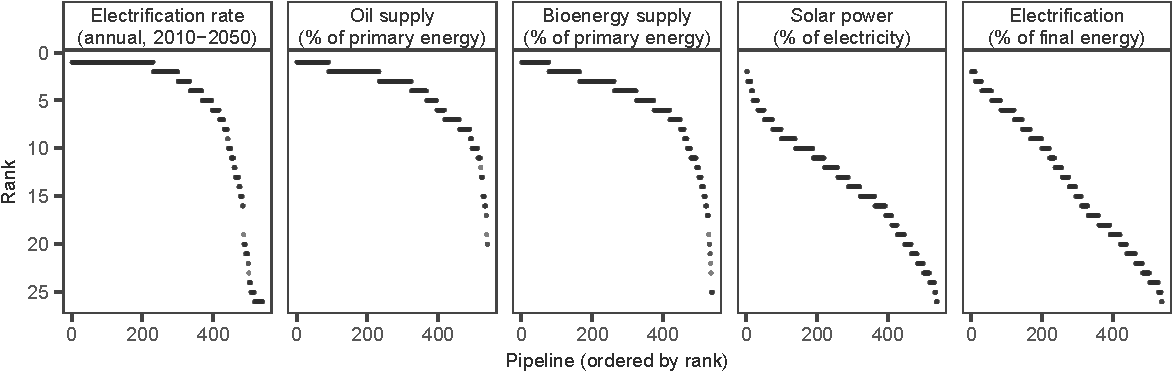
\includegraphics[width=0.8\textwidth]{spec-curve-1.png}
    \caption{Ranking of five of the key decarbonization measures proposed by \cite{Li_Pye_Keppo_Jaxa-Rozen_Trutnevyte_2023} after running them through a garden of c. 540 different paths.}
    \label{fig:RankingKey}
\end{figure}

As shown in Figure \ref{fig:RankingKey} solar power is never the top lever in any of the 540 paths (its rank spans 2 to 26, median of 13). Same for electrification. 



\section{Giulia's analysis: replicating Li et al.}


\cite{Li_Pye_Keppo_Jaxa-Rozen_Trutnevyte_2023} propose a three-stage pipeline to identify the regional decarbonisation measures most influential in reaching the 2\textdegree C and 1.5\textdegree C targets, applied to the public IPCC SR1.5 scenario database (411 scenarios, 19 IAMs, 5 aggregated world regions). The
pipeline proceeds as follows:

\begin{enumerate}
	\item \textbf{Metric selection and pre-screening.} $\sim$26 regional metrics (technology shares, an energy-intensity ratio, and annual growth rates) are extracted for each of the 5 regions ($\sim$130 metrics in total). Pairwise Pearson correlation is computed across all metrics, and one representative metric is kept from each group exceeding a correlation threshold of 0.85: ``the first one from each group of highly correlated metrics.''
	\item \textbf{Random Forest.} A Random Forest classifier is fitted on the 3-category temperature target (Above 2\textdegree C / 2\textdegree C /1.5\textdegree C), separately for structure/ratio metrics and for growth-rate metrics, with hyperparameters (n\_estimators, max\_depth, max\_samples) selected via a 1,000-combination grid search on a fresh 80/20 train/test split each time, keeping the combination with the highest test
	accuracy (96\% for structure metrics, 83\% for growth-rate metrics). Metrics are ranked by Gini importance; those with cumulative importance up
	to 0.8 are retained.
	\item \textbf{Logistic regression.} A logistic regression model is fitted on two binary targets (below 2\textdegree C, below 1.5\textdegree C) using
	the RF-selected metrics, repeated over 10 random 80/20 splits, to rank and sign each metric's average influence (Fig.~6).
	\item \textbf{PRIM.} The Patient Rule Induction Method is applied to the RF-selected metrics to identify ``boxes'', that are combinations of metric ranges  associated with each temperature category, restricted to 3 metrics per	box ``for simplicity,'' and accepted when recall or precision exceeds 0.9
	and F1 exceeds 0.7 (Fig.~7).
\end{enumerate}

Headline claims (Abstract; Conclusions \S5): solar power and sectoral electrification are the most influential measures across all regions; unabated gas phase-out and energy efficiency improvement are additionally crucial for 1.5\textdegree C; bioenergy (especially in Latin America) and wind show more regional heterogeneity.

\subsection{Issues found in exact replication}

No code accompanies the paper; the replication below (R and Python) follows the method exactly as described in the manuscript and appendices. Data fidelity was validated first: medians of three key metrics (PriBio, EngInt.Ratio, FinElc) by region and temperature category match Figs.~2--3 closely across all 15 region$\times$category combinations tested, so the issues below are not a data problem.

\begin{enumerate}
	\item \textbf{The reported 96\% RF accuracy is very likely an artefact of the tuning procedure, not a stable model property.} Accuracy checked four independent ways (R and Python OOB estimates, a stratified 80/20 test-set average over 10 splits, and a direct simulation of the paper's own 1,000-combination grid search) all converge on $\sim$83--86\%. Simulating their exact procedure (1,000 random hyperparameter draws, a fresh 80/20 split each time, keeping the maximum observed test accuracy) reproduces 95.4\%, matching their reported figure almost exactly: mean = 83.6\%, max = 95.4\%. This is a selection bias / winner's curse: taking the best of many noisy accuracy draws systematically overstates the true, stable accuracy of the model.
	\item \textbf{The logistic regression is very likely L2-regularised (Ridge), not the plain maximum-likelihood method the text describes.}
	Replicating the method literally (plain logistic regression, $\sim$30 metrics from the 0.8 cumulative-importance threshold) produces
	near-perfect separation and coefficients of order $10^{15}$. \texttt{scikit-learn}'s \texttt{LogisticRegression} applies L2
	regularisation by default (confirmed in the package documentation), and the paper never states this was disabled. Switching to Ridge resolves the
	separation and yields coefficients consistent in sign and relative magnitude with Fig.~6.
	\item \textbf{The correlation threshold (0.85) is declared; the tie-break rule is not.} The paper specifies the 0.85 threshold explicitly, but gives no criterion for how ``the first one from each group of highly correlated metrics'' is ordered, that is an undeclared degree of freedom, distinct from the threshold value itself.
	\item \textbf{An unexplained driver absent from the paper's own results.} \texttt{PriOil} (share of oil in primary energy), available in the
	authors' own metric set (Appendix C) but never discussed or shown in Fig.~5,  ranks among the top-2 most important structure metrics in our Random Forest, regardless of correlation threshold or of whether the full 85-column structure/ratio pool is used with no screening 	at all. Ruled out: correlation-driven tie-break exclusion (its strongest correlation with any retained metric is $-0.80$, below the 0.85 threshold) and pool-size dilution (it remains dominant even with maximal
	competing metrics). Root cause not identified without the original code; flagged as a second concrete instance of instability in the original
	pipeline, independent of the winner's curse finding above.
	\item \textbf{The PRIM box selection criterion is under-determined.} The acceptance rule (recall or precision $>0.9$, combined with F1 $>0.7$) is satisfied by multiple points along a given peeling trajectory, not a single one; the paper does not specify how this is resolved (first qualifying point? maximum F1?). Treated in our GSA design as an additional factor rather than fixed by assumption.
\end{enumerate}

\subsection{GSA setting}

 Each headline claim was translated into an operational rule verifiable on the pipeline's output, since the paper itself states these findings qualitatively, without a declared numerical threshold.

\subsubsection{Claims and their operational rules}

\begin{enumerate}
\item[C1a] \textit{``electrification level (FinElc)... have been found the most influential in limiting global temperature increases''} (Sec.~4.3). \textbf{Rule}: FinElc (any region) is among the 3 metrics with the largest \emph{positive} coefficient in the logistic regressions.
\item[C1b] \textit{``solar power generation (ElcSol)... have been found the most influential''} (Sec.~4.3). \textbf{Rule}: at least one of ElcSol/ElcWnd/ElcNuc is among the 3 metrics with the largest positive coefficient. Solar, wind and nuclear are pooled because none of the three individually survives the pipeline consistently enough across factor combinations to be tested alone.
	\item[C1] \textit{``solar power and sectoral electrification... found to be the most effective measures''} (Abstract). \textbf{Rule}: C1a AND C1b hold
	jointly in the same run.
	\item[C2] \textit{``unabated gas usage... see high negative coefficients''} (Sec.~4.3); \textit{``decommissioning of unabated gas plants should be prioritised''} (Conclusions \S5.1). \textbf{Rule}: ElcGas or PriGas (any region) is among the 3 most negative coefficients.
	\item[C3] \textit{``energy intensity (EngInt.Ratio)... has been shown to be more influential than most supply-side measures''} (Sec.~4.3). \textbf{Rule}: EngInt.Ratio is among the 3 most negative coefficients.
\item[C4] \textit{``bioenergy supply... LAM being the most influential region''} (Sec.~4.3); \textit{``primary bioenergy supply in LAM is particularly influential''} (Conclusions \S5.3--4). \textbf{Rule}: among metrics restricted to the LAM region, PriBio has the largest \emph{positive} coefficient.
	\item[C5] PRIM box for 1.5\textdegree C (Sec.~4.4, Fig.~7 bottom): ElcGas $<$5.2\%, EngInt.Ratio $<$56\%, FinElc $>$36\%, P=0.56, R=0.98. \textbf{Rule}: the box selected along our manual peeling trajectory (first point satisfying recall$>$0.9 OR precision$>$0.9, AND F1$>$0.7) has precision$>$0.45 and recall$>$0.85: acceptance thresholds relaxed from the paper's own P/R to tolerate variation across runs while retaining a minimal validity bar.
\end{enumerate}

Note: the original claim about ``solar power and sectoral electrification", as stated in the Abstract (\textit{``solar power and sectoral electrification... found to be the most effective measures''}), was initially used as a single joint rule (FinElc AND at least one of ElcSol/ElcWnd/ElcNuc among the top coefficients). Under this joint rule the claim held in essentially none of the runs tested manually, which on inspection was driven entirely by one of its two components: FinElc was present among the top coefficients in the large majority of runs, while ElcSol/ElcWnd/ElcNuc almost never was. Collapsing both halves into a single pass/fail obscured this asymmetry: a low joint success rate could equally have meant both components were fragile or, as turned out to be the case, only one of them was. The claim was therefore split into C1a (electrification alone) and C1b (low-carbon generation alone), with C1 retained as their conjunction, so that the source of the joint claim's fragility is directly visible rather than averaged away.

\subsubsection{Factors and perturbation}


Twelve factors were varied via Sobol' quasi-random sequences
(\texttt{sensobol}, $N=4096$, first-order estimator \texttt{"saltelli"} and
total-order estimator \texttt{"jansen"}, $R=1000$ bootstrap replicates; Table~\ref{tab:gsa_factors}).

\begin{table}[h]
	\centering
	\caption{Factors varied in the Sobol' design (F8, F13, F14 currently held
		fixed: open to discussion whether to include them as additional factors. Note: $^{*}$The paper's own grid search (Appendix E) does test a range of
		max\_depth values (1--19) before selecting a single best value (9 or 5); but \texttt{randomForest} in R has no direct max\_depth equivalent to
		scikit-learn's, so their tested range cannot be reproduced as such, and \texttt{nodesize} is used as an inverse-order proxy instead.}
	\begin{tabular}{@{}lll@{}}
		\toprule
		Factor & Paper's value & Range tested \\
		\midrule
		F1  & Correlation threshold: 0.85                            & 0.5--0.9 \\
		F2  & Correlation tie-break rule: unspecified                & first-in-order / max-variance \\
		F3  & n\_estimators: tested grid 50--1000                    & 50--1000 \\
		F4  & max\_depth: grid tested 1--19, single value selected$^{*}$ & \texttt{nodesize} $\in \{1,2,3,5,7,10,15,20,30,50\}$ \\
		F5  & max\_samples: tested grid 0.5--0.9                     & 0.5--0.9 \\
		F6  & Importance metric: Gini only                           & Gini / permutation \\
		F7  & Cumulative importance threshold: 0.8                   & 0.5--0.9 \\
		F9.1 & Train fraction: 0.8                                   & 0.5--0.85 \\
		F9.2 & Number of repeats: 10                                 & 10--30 \\
		F10 & Metrics per PRIM box: 3 (``for simplicity'')           & 2--5 \\
		F11 & PRIM recall/precision threshold: 0.9                   & 0.7--0.9 \\
		F12 & PRIM F1 threshold: 0.7                                 & 0.6--0.9 \\
		\bottomrule
	\end{tabular}
		\label{tab:gsa_factors}
\end{table}


\subsection{Results}

The GSA reported here concerns both the below-1.5\textdegree C target (claims C1a--C5) and, for six of the seven claims, the below-2\textdegree C target (claims C1a\_2C--C4\_2C); C5\_2C is omitted, as it would require duplicating the PRIM stage on the below-2\textdegree C target. Across the full Sobol' design ($N=4096$, 57{,}344 runs), the fraction of runs in which each claim holds is reported in Table~\ref{tab:claim_fractions} and Fig.~\ref{fig:claim_fractions}.

\begin{table}[h]
	\centering
	\caption{Fraction of runs (out of 57,344) in which each claim holds, both targets.}
	\label{tab:claim_fractions}
	\begin{tabular}{@{}lcc@{}}
		\toprule
		Claim & below 1.5\textdegree C & below 2\textdegree C \\
		\midrule
		C1a (electrification)       & 67.7\% & 62.9\% \\
		C1b (low-carbon generation) & 25.0\% & 12.7\% \\
		C1 (joint, as stated)       & 7.8\%  & 4.3\%  \\
		C2 (gas phase-out)          & 25.4\% & 42.6\% \\
		C3 (energy efficiency)      & 65.2\% & 83.0\% \\
		C4 (LAM bioenergy)          & 40.3\% & 74.7\% \\
		C5 (PRIM box)               & 15.0\% & --- \\
		\bottomrule
	\end{tabular}
\end{table}

\begin{figure}[h]
	\centering
	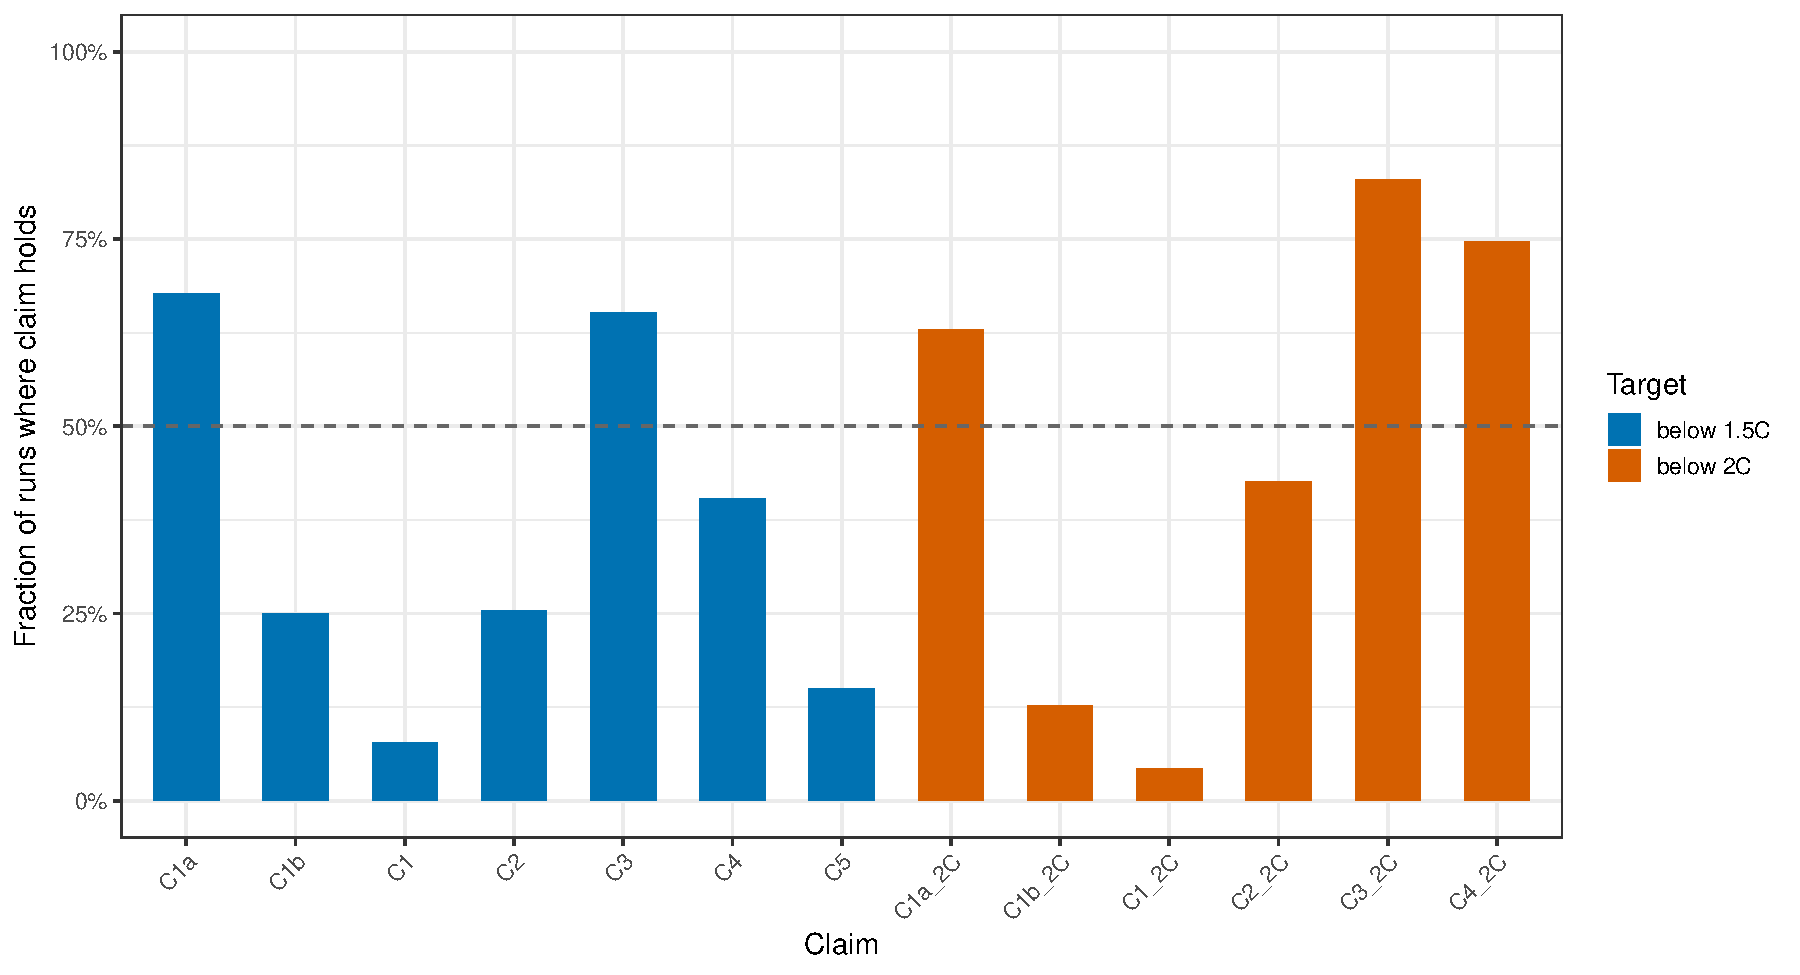
\includegraphics[width=\textwidth]{Figure/claim_fractions_with2C.pdf}
	\caption{Fraction of the 57,344 Sobol' runs in which each claim holds, below-1.5\textdegree C (blue) and below-2\textdegree C (orange).}
	\label{fig:claim_fractions}
\end{figure}

Only two of the seven below-1.5\textdegree C claims hold in a majority of runs (C1a, C3); the paper's own headline claim, taken jointly as stated in the Abstract (C1), holds in under 8\% of runs. Shifting to the below-2\textdegree C target does not uniformly stabilise or destabilise these claims: C1a, C1b and C1 become \emph{less} robust (C1b nearly halves, from 25.0\% to 12.7\%), while C2, C3 and C4 become \emph{substantially more} robust (i.e. C4 (LAM bioenergy) nearly doubles,
from 40.3\% to 74.7\%). Which conclusions appear solid therefore depends systematically on which temperature threshold is chosen, not only on which analyst choices are made within a fixed threshold.

Sobol' total-order indices (Fig.~\ref{fig:sobol_indices}; full results in the Supplementary Tables, Appendix~\ref{app:sobol_tables}) show that this instability is concentrated in two factors across nearly all claims. F1
(the correlation threshold) and F7 (the cumulative importance threshold), two choices both declared by the paper as fixed values, and treated here as ordinary methodological choices, are jointly the dominant factors for twelve of the thirteen claims tested (Table~\ref{tab:sobol_ti}).

\begin{table}[h]
	\centering
	\caption{Dominant factors by total-order Sobol' index ($T_i$, Jansen estimator, $N=4096$, $R=1000$ bootstrap).}
	\label{tab:sobol_ti}
	\begin{tabular}{@{}lll@{}}
		\toprule
		Claim & 1st factor ($T_i$) & 2nd factor ($T_i$) \\
		\midrule
		C1a & F1 (0.845) & F2 (0.587) \\
		C1b & F1 (0.829) & F7 (0.718) \\
		C1  & F1 (0.968) & F2 (0.812) \\
		C2  & F7 (0.740) & F1 (0.647) \\
		C3  & F1 (0.907) & F7 (0.677) \\
		C4  & F7 (0.685) & F1 (0.647) \\
		C5  & F12 (0.927) & F1 (0.654) \\
		C1a\_2C & F1 (0.886) & F2 (0.636) \\
		C1b\_2C & F1 (0.941) & F7 (0.789) \\
		C1\_2C  & F1 (0.972) & F7 (0.851) \\
		C2\_2C  & F7 (0.729) & F1 (0.680) \\
		C3\_2C  & F1 (0.818) & F7 (0.731) \\
		C4\_2C  & F1 (0.927) & F2 (0.637) \\
		\bottomrule
	\end{tabular}
\end{table}

\begin{figure}[h]
	\centering
	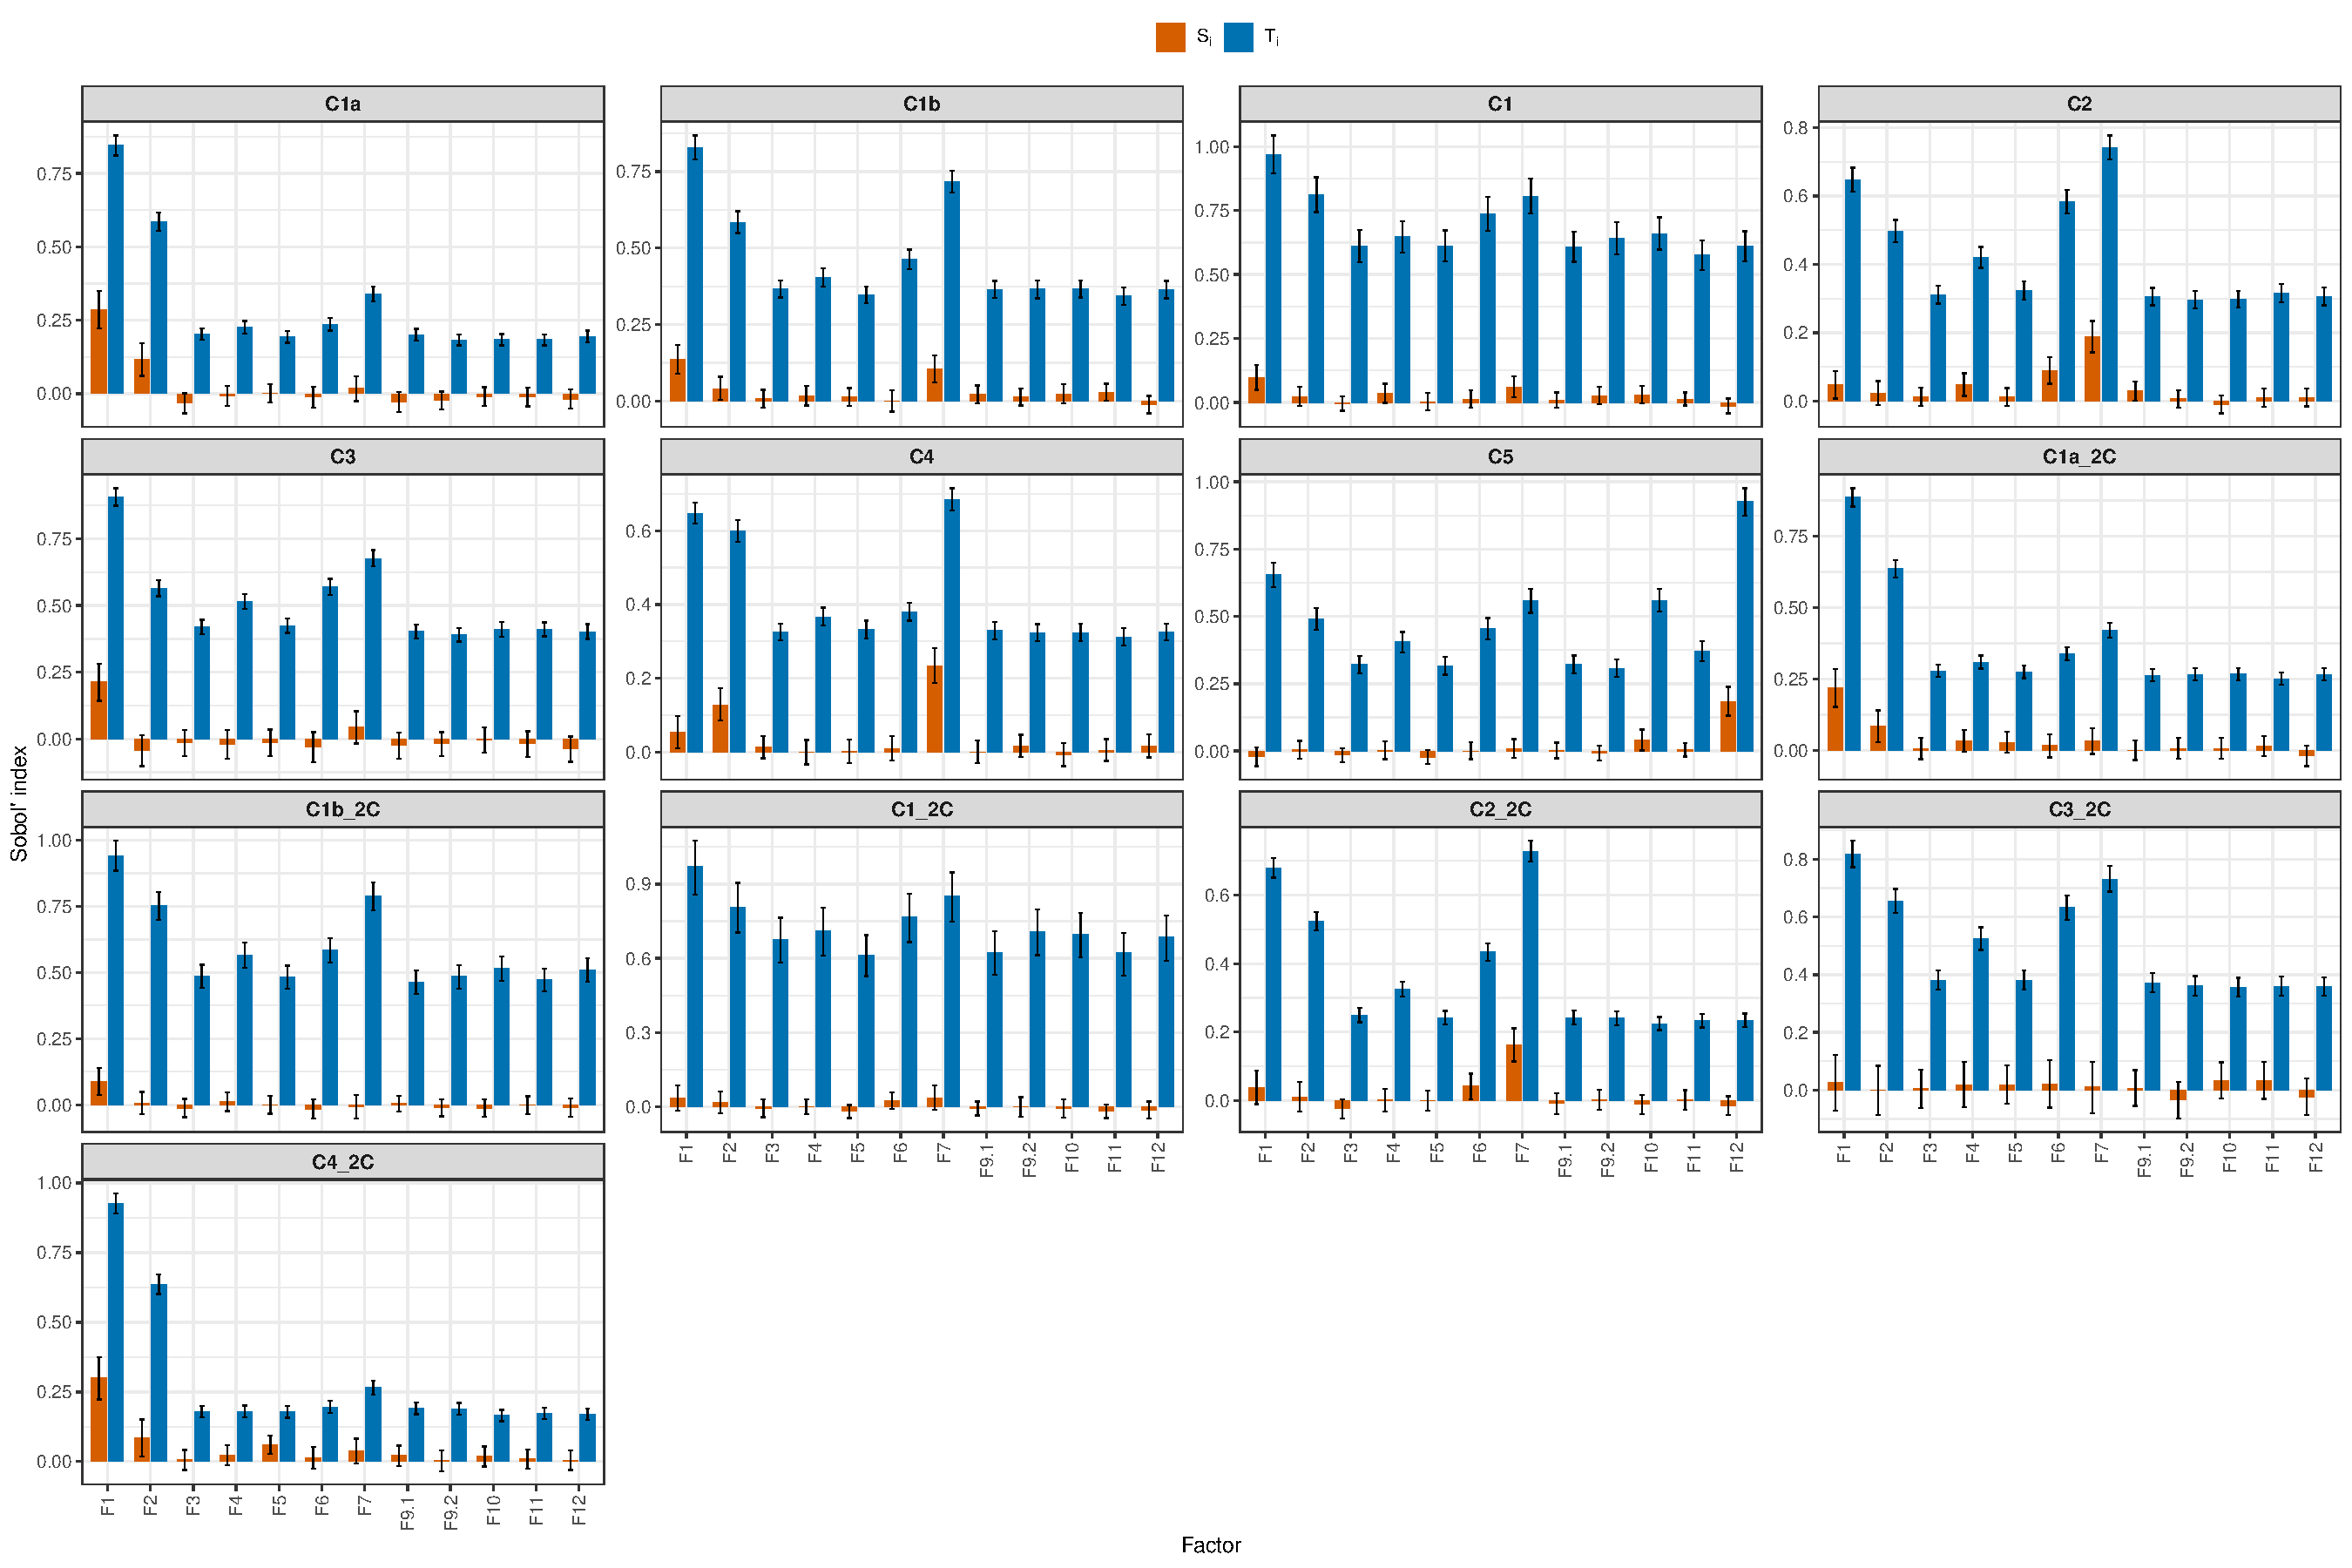
\includegraphics[width=\textwidth]{Figure/sobol_indices_all_claims_with2C.pdf}
	\caption{First-order ($S_i$, Saltelli estimator) and total-order ($T_i$, Jansen estimator) Sobol' indices for each of the twelve factors, by claim. Error bars show 95\% bootstrap confidence intervals.}
	\label{fig:sobol_indices}
\end{figure}

In every case, first-order indices are markedly smaller than the corresponding total-order indices, suggesting that instability is carried predominantly by interactions among factors, not by any single factor acting in isolation. The correlation tie-break rule (F2, itself undeclared by the paper) also contributes non-trivially as a secondary factor for six of the thirteen claims, alongside F1 and F7.

To summarize, the paper's headline claim that solar power and electrification are jointly the most
influential measures (C1) is almost entirely driven by its electrification half (C1a); the low-carbon generation half (C1b) rarely survives the pipeline regardless of the factors perturbed, for either temperature target. Second, and independently of this instability, a metric absent from the paper's own discussion (\texttt{PriOil}) consistently displaces both \texttt{EngInt.Ratio} and \texttt{PriBio} from the top of the ranking under the paper's own declared correlation threshold, suggesting the
published ranking may itself depend on a specific, undocumented selection of scenarios or metrics not recoverable from the text alone.





\section{Discussion}

\subsection{What is new in this work respect to previous sensitivity analyses}
\textcolor{red}{Global sensitivity analysis has been applied to IAMs before, but always to the \emph{model}: one varies the model's physical and economic inputs and asks which drive its outputs \citep{Chiani_Borgonovo_Plischke_Tavoni_2025}. Our object is different and one level up. We hold the scenario-discovery \emph{procedure} as the object of analysis, take the analyst's methodological choices --- classifier, importance metric, temperature-binning, PRIM thresholds --- as the input factors, and take the discovered driver-ranking as the output. We audit not the climate--economy model but the epistemic apparatus laid over its ensemble; to our knowledge this is the first such analysis.}

\textcolor{red}{The distinction sharpens a complaint already voiced within our community.} The central methodological complaint of \cite{Chiani_Borgonovo_Plischke_Tavoni_2025} is that IAM
sensitivity work collapses a multivariate emissions trajectory into a scalar,
and that this is unsatisfactory. This is also true of scenario discovery. PRIM and random-forest classifiers reduce the entire pathway
to a binary label (``reaches 1.5\,\textdegree C by 2100: yes/no'') and then
hunt for drivers of that scalar. If they are right that scalarising the
trajectory throws away decision-relevant structure, then scenario discovery,
which scalarises even harder --- to one bit --- discards still more, and the
``drivers'' it finds are drivers of an arbitrary thresholding choice. 


\subsection{Measuring uncertainty without acting on it}
Crucially, and somewhat paradoxically, sensitivity analysis is given more leverage than uncertainty analysis: while the differing sensitivities of different input assumptions become an occasion for reflection on the technical or normative quality of the inference, the plain existence of large uncertainties does not trigger a warning against using the inference for policy --- a posture of ``uncertainty quantified, let us move on to interpret the results'' where the honest reading is ``no point interpreting these results given the uncertainties.''

\subsection{Link to composite indicator}
The critique of
collapsing a multivariate object into a single figure of merit is one we have
made before, in the setting of composite indicators: the illusory precision of
rankings built by aggregation \cite{paruolo_ratings_2013}, and the
methodological cautions of the OECD--JRC handbook on composite indicator
construction \cite{oecd_oecd-jrc_2008}. The same objection --- that the weighting
and aggregation choices, not the underlying evidence, drive the resulting
order --- transfers directly to the temperature-binning and thresholding of
scenario discovery.

\subsection{The scenario discovery pipeline through the lens of philosophy of models}

\textcolor{red}{The instability our Sobol' indices quantify is not a numerical curiosity; it is what one should expect from a representational apparatus whose fidelity is never secured. The philosophy of models makes this precise, and gives the reordering of drivers under analyst choice its interpretation: a pipeline can identify a region for reasons unrelated to the causal structure of its target --- exactly the failure of ``representational fidelity'' below.}

Scenario discovery is not a model in the conventional sense but a \textit{pipeline} --- a sequence of computational steps (sampling, simulation, classification, feature identification) that transforms a space of assumptions into a set of policy-relevant scenarios. Yet the pipeline, taken as a whole, functions \textit{as} a model: it takes inputs (assumptions about a system), operates on them through a formal apparatus, and produces outputs (scenarios, vulnerability regions, importance rankings) that are taken to represent something about the world. If this is right, then the tools developed by philosophers of models to analyse representation can be applied to the pipeline itself --- not only to its individual components.

Michael Weisberg's \textit{Simulation and Similarity} \citep{weisberg_simulation_2013} provides the most systematic framework for this purpose. For Weisberg, a model represents its target not by virtue of any intrinsic resemblance but through a \textit{construal} --- a set of specifications, supplied by the modeller, that determines how the model is to be read as a representation. The construal has four elements:

\begin{enumerate}
    \item \textbf{Assignment}: which real-world system the model targets --- what in the world the model is \textit{about}.
    \item \textbf{Scope}: what class of systems or phenomena the model aims to cover --- the breadth of its intended applicability.
    \item \textbf{Dynamical fidelity}: does the model predict well? --- the accuracy of its outputs relative to observations.
    \item \textbf{Representational fidelity}: does the model predict well \textit{for the right reasons}? --- whether the mechanisms it embodies correspond to those operating in the target system.
\end{enumerate}

Weisberg illustrates these with the Lotka-Volterra model applied to a fisheries case study. The \textit{assignment} is the Adriatic sardine population. The \textit{scope} is small pelagic species under moderate exploitation regimes --- the class of systems for which the model's assumptions are considered applicable. \textit{Dynamical fidelity} asks whether the model's predictions match observed population dynamics. \textit{Representational fidelity} asks the harder question: does it get the dynamics right for the right reasons?

Applied to the scenario discovery pipeline as a whole, each element takes on a specific form:

\textit{Assignment.} What does the pipeline's output --- a set of scenarios labelled `vulnerable' or `robust', a ranking of input factors by importance. The assignment is doubly mediated: by the simulation model's own representational choices and by the classification algorithm's thresholds.

\textit{Scope.} The pipeline inherits the scope of the underlying simulation but adds a further restriction: it explores only those dimensions of uncertainty that the analyst has chosen to sample. 

\textit{Dynamical fidelity.} Does the pipeline predict well? For a simulation model, this can in principle be assessed against observations. For the pipeline, there is no direct observational test --- the output is a partitioning of an input space, not a prediction of an observable quantity. Dynamical fidelity must therefore be assessed indirectly: does the classification capture the right regions? Does the importance ranking remain stable under perturbation? These questions have no standard answers, and the pipeline offers no internal mechanism to generate them.

\textit{Representational fidelity.} Does the pipeline get the answer for the right reasons? A classification algorithm may correctly identify a vulnerability region but for reasons that have nothing to do with the causal structure of the problem --- an artefact of the sampling scheme, a threshold effect in the classifier, a spurious correlation in high-dimensional input space. 

Weisberg's four elements reveal the complexity of the pipeline's representational claim. But the construal, even fully specified, remains incomplete. It tells us \textit{what} the pipeline targets, over \textit{what} scope, and at \textit{what} level of fidelity. It does not tell us \textit{by whom} and \textit{for whom}. To go back to the sardine example, a model developed by the syndicate of the lagoon's fishermen is likely different from one developed by a food conglomerate.

This is where Charles Sanders Peirce's triadic semiotics becomes indispensable \citep{saltelli_equations_2026, boulanger_elements_2014}. For Peirce, representation is never a dyadic relation between sign and object; it is irreducibly triadic, requiring a sign (here, the pipeline's output), an object (the target system), and an \textit{interpretant} --- the meaning produced in an interpreter who reads the sign in relation to its object and acts upon it. Without the interpretant, no representation occurs; the pipeline is an artefact without a reader, formally complete but devoid of agency.

The interpretant functions as a \textbf{fifth element of the construal}:

\begin{enumerate}
    \setcounter{enumi}{4}
    \item \textbf{Interpretant}: The action suggested or implied by the pipeline; its `end in view', the behaviour that the sign is supposed to activate in the recipient of the message.
\end{enumerate}

Without the interpretant, the other four elements are specifications without a reader --- instructions that no one follows. With it, the pipeline becomes part of a chain of human judgments that determine what actions should be taken following the pipeline's inference. The question of the interpretant is therefore not a philosophical addendum to the analysis of scenario discovery but its most consequential element, loaded as it is with policy prescriptions, for example of climate mitigation or energy transition, considered as desirable. 




\section{Conclusions}
Our conclusion is that 
signals scenario discovery reads are real --- but they are signals about the construction of the ensemble, not about the world. If the ensemble spread is
dominated by structural and parametric choices rather than by anything
decision-relevant, the ``features that lead to decarbonisation'' are artefacts
of the design: the analyst's own choices handed back to him.


\section{Journals}\textit{Environmental Modelling \& Software} is a first thought for a safe and possibly rapid home. You may not like it, but this a journal these communities actually read. In my experience, journals in the \textit{Nature} family would vigorously push back on the pushback. If one wants to take the risk, then \textit{Nature Climate Change} is a possibility, but I would send a pre-inquiry beforehand, so as not to waste our time.


\section{Acknowledgments}
AS acknowledges the inspiration for the present work from a recent school
\citep{university_of_geneva_prisma_2026} where participants were trained to
explore IPCC-class scenario ensembles for the features that lead, or fail to
lead, to decarbonisation by 2070 --- the school's own programmatic horizon.

%\bibliographystyle{sn-basic}
%\bibliographystyle{sn-mathphys-num}
\bibliography{bibliography}

\appendix
\section{Supplementary Tables: Complete Sobol' Indices}
\label{app:sobol_tables}

Tables below report the complete first-order ($S_i$, Saltelli estimator) and total-order ($T_i$, Jansen estimator) Sobol' indices, with 95\% bootstrap confidence intervals ($R=1000$), for all twelve factors and all thirteen claims.

% latex table generated in R 4.6.1 by xtable 1.8-8 package
% Wed Aug  5 13:46:48 2026
\begin{table}[ht]
\centering
\caption{Sobol' indices for claim C1a ($N=4096$, Saltelli estimator for $S_i$, Jansen for $T_i$, 95\% bootstrap CI in parentheses).} 
\label{tab:sobol_C1a}
\begin{tabular}{lll}
  \hline
Factor & Si & Ti \\ 
  \hline
F1 & 0.287 (0.223, 0.351) & 0.845 (0.811, 0.879) \\ 
  F2 & 0.116 (0.061, 0.171) & 0.587 (0.555, 0.617) \\ 
  F3 & -0.032 (-0.067, 0.001) & 0.203 (0.183, 0.223) \\ 
  F4 & -0.007 (-0.042, 0.026) & 0.226 (0.205, 0.247) \\ 
  F5 & 0.002 (-0.030, 0.033) & 0.193 (0.174, 0.213) \\ 
  F6 & -0.011 (-0.047, 0.024) & 0.237 (0.215, 0.259) \\ 
  F7 & 0.018 (-0.025, 0.060) & 0.339 (0.315, 0.364) \\ 
  F9.1 & -0.028 (-0.063, 0.006) & 0.201 (0.181, 0.221) \\ 
  F9.2 & -0.023 (-0.054, 0.007) & 0.183 (0.165, 0.202) \\ 
  F10 & -0.009 (-0.041, 0.022) & 0.184 (0.165, 0.203) \\ 
  F11 & -0.010 (-0.043, 0.021) & 0.184 (0.164, 0.202) \\ 
  F12 & -0.018 (-0.051, 0.015) & 0.196 (0.175, 0.215) \\ 
   \hline
\end{tabular}
\end{table}

% latex table generated in R 4.6.1 by xtable 1.8-8 package
% Wed Aug  5 13:46:48 2026
\begin{table}[ht]
\centering
\caption{Sobol' indices for claim C1b ($N=4096$, Saltelli estimator for $S_i$, Jansen for $T_i$, 95\% bootstrap CI in parentheses).} 
\label{tab:sobol_C1b}
\begin{tabular}{lll}
  \hline
Factor & Si & Ti \\ 
  \hline
F1 & 0.137 (0.089, 0.184) & 0.829 (0.790, 0.867) \\ 
  F2 & 0.041 (0.003, 0.080) & 0.584 (0.549, 0.620) \\ 
  F3 & 0.008 (-0.021, 0.037) & 0.366 (0.338, 0.394) \\ 
  F4 & 0.018 (-0.015, 0.050) & 0.404 (0.374, 0.435) \\ 
  F5 & 0.013 (-0.015, 0.042) & 0.347 (0.319, 0.374) \\ 
  F6 & 0.000 (-0.034, 0.035) & 0.462 (0.431, 0.495) \\ 
  F7 & 0.105 (0.061, 0.149) & 0.718 (0.681, 0.752) \\ 
  F9.1 & 0.022 (-0.007, 0.051) & 0.364 (0.336, 0.392) \\ 
  F9.2 & 0.013 (-0.015, 0.041) & 0.366 (0.336, 0.394) \\ 
  F10 & 0.024 (-0.008, 0.055) & 0.366 (0.338, 0.395) \\ 
  F11 & 0.027 (0.001, 0.057) & 0.343 (0.314, 0.371) \\ 
  F12 & -0.012 (-0.040, 0.017) & 0.364 (0.335, 0.392) \\ 
   \hline
\end{tabular}
\end{table}

% latex table generated in R 4.6.1 by xtable 1.8-8 package
% Wed Aug  5 13:46:48 2026
\begin{table}[ht]
\centering
\caption{Sobol' indices for claim C1 ($N=4096$, Saltelli estimator for $S_i$, Jansen for $T_i$, 95\% bootstrap CI in parentheses).} 
\label{tab:sobol_C1}
\begin{tabular}{lll}
  \hline
Factor & Si & Ti \\ 
  \hline
F1 & 0.098 (0.049, 0.147) & 0.968 (0.894, 1.043) \\ 
  F2 & 0.024 (-0.013, 0.062) & 0.812 (0.744, 0.880) \\ 
  F3 & -0.003 (-0.032, 0.025) & 0.612 (0.549, 0.674) \\ 
  F4 & 0.037 (-0.001, 0.073) & 0.647 (0.587, 0.709) \\ 
  F5 & 0.003 (-0.030, 0.037) & 0.612 (0.552, 0.673) \\ 
  F6 & 0.014 (-0.019, 0.047) & 0.737 (0.672, 0.803) \\ 
  F7 & 0.061 (0.021, 0.102) & 0.807 (0.739, 0.874) \\ 
  F9.1 & 0.010 (-0.019, 0.040) & 0.608 (0.550, 0.668) \\ 
  F9.2 & 0.027 (-0.006, 0.061) & 0.641 (0.578, 0.704) \\ 
  F10 & 0.031 (-0.004, 0.065) & 0.659 (0.598, 0.723) \\ 
  F11 & 0.014 (-0.012, 0.040) & 0.578 (0.519, 0.634) \\ 
  F12 & -0.014 (-0.043, 0.016) & 0.610 (0.551, 0.669) \\ 
   \hline
\end{tabular}
\end{table}

% latex table generated in R 4.6.1 by xtable 1.8-8 package
% Wed Aug  5 13:46:48 2026
\begin{table}[ht]
\centering
\caption{Sobol' indices for claim C2 ($N=4096$, Saltelli estimator for $S_i$, Jansen for $T_i$, 95\% bootstrap CI in parentheses).} 
\label{tab:sobol_C2}
\begin{tabular}{lll}
  \hline
Factor & Si & Ti \\ 
  \hline
F1 & 0.047 (0.007, 0.088) & 0.647 (0.612, 0.683) \\ 
  F2 & 0.024 (-0.012, 0.058) & 0.497 (0.464, 0.530) \\ 
  F3 & 0.013 (-0.014, 0.039) & 0.311 (0.285, 0.338) \\ 
  F4 & 0.048 (0.015, 0.081) & 0.421 (0.390, 0.451) \\ 
  F5 & 0.013 (-0.013, 0.038) & 0.324 (0.297, 0.350) \\ 
  F6 & 0.089 (0.051, 0.128) & 0.584 (0.549, 0.618) \\ 
  F7 & 0.187 (0.142, 0.234) & 0.740 (0.706, 0.777) \\ 
  F9.1 & 0.030 (0.002, 0.057) & 0.306 (0.280, 0.331) \\ 
  F9.2 & 0.007 (-0.020, 0.032) & 0.296 (0.271, 0.321) \\ 
  F10 & -0.009 (-0.036, 0.017) & 0.298 (0.273, 0.322) \\ 
  F11 & 0.010 (-0.017, 0.037) & 0.315 (0.289, 0.342) \\ 
  F12 & 0.010 (-0.016, 0.036) & 0.306 (0.280, 0.332) \\ 
   \hline
\end{tabular}
\end{table}

% latex table generated in R 4.6.1 by xtable 1.8-8 package
% Wed Aug  5 13:46:48 2026
\begin{table}[ht]
\centering
\caption{Sobol' indices for claim C3 ($N=4096$, Saltelli estimator for $S_i$, Jansen for $T_i$, 95\% bootstrap CI in parentheses).} 
\label{tab:sobol_C3}
\begin{tabular}{lll}
  \hline
Factor & Si & Ti \\ 
  \hline
F1 & 0.213 (0.143, 0.281) & 0.907 (0.874, 0.940) \\ 
  F2 & -0.042 (-0.102, 0.015) & 0.565 (0.535, 0.595) \\ 
  F3 & -0.015 (-0.065, 0.032) & 0.420 (0.392, 0.447) \\ 
  F4 & -0.020 (-0.073, 0.034) & 0.515 (0.486, 0.544) \\ 
  F5 & -0.014 (-0.064, 0.035) & 0.424 (0.398, 0.451) \\ 
  F6 & -0.032 (-0.088, 0.025) & 0.570 (0.539, 0.600) \\ 
  F7 & 0.044 (-0.017, 0.104) & 0.677 (0.647, 0.708) \\ 
  F9.1 & -0.024 (-0.074, 0.024) & 0.403 (0.377, 0.428) \\ 
  F9.2 & -0.019 (-0.064, 0.026) & 0.390 (0.365, 0.415) \\ 
  F10 & -0.003 (-0.053, 0.044) & 0.410 (0.382, 0.438) \\ 
  F11 & -0.017 (-0.067, 0.029) & 0.411 (0.384, 0.437) \\ 
  F12 & -0.037 (-0.086, 0.009) & 0.402 (0.375, 0.430) \\ 
   \hline
\end{tabular}
\end{table}

% latex table generated in R 4.6.1 by xtable 1.8-8 package
% Wed Aug  5 13:46:48 2026
\begin{table}[ht]
\centering
\caption{Sobol' indices for claim C4 ($N=4096$, Saltelli estimator for $S_i$, Jansen for $T_i$, 95\% bootstrap CI in parentheses).} 
\label{tab:sobol_C4}
\begin{tabular}{lll}
  \hline
Factor & Si & Ti \\ 
  \hline
F1 & 0.053 (0.011, 0.097) & 0.647 (0.620, 0.676) \\ 
  F2 & 0.128 (0.085, 0.173) & 0.599 (0.571, 0.629) \\ 
  F3 & 0.013 (-0.017, 0.044) & 0.326 (0.303, 0.349) \\ 
  F4 & -0.001 (-0.034, 0.032) & 0.367 (0.343, 0.392) \\ 
  F5 & 0.001 (-0.030, 0.033) & 0.332 (0.308, 0.356) \\ 
  F6 & 0.009 (-0.024, 0.043) & 0.380 (0.356, 0.405) \\ 
  F7 & 0.234 (0.187, 0.282) & 0.685 (0.655, 0.715) \\ 
  F9.1 & 0.000 (-0.030, 0.031) & 0.329 (0.306, 0.352) \\ 
  F9.2 & 0.015 (-0.014, 0.047) & 0.323 (0.301, 0.347) \\ 
  F10 & -0.007 (-0.038, 0.024) & 0.324 (0.301, 0.347) \\ 
  F11 & 0.005 (-0.025, 0.035) & 0.312 (0.289, 0.335) \\ 
  F12 & 0.015 (-0.015, 0.048) & 0.325 (0.303, 0.347) \\ 
   \hline
\end{tabular}
\end{table}

% latex table generated in R 4.6.1 by xtable 1.8-8 package
% Wed Aug  5 13:46:48 2026
\begin{table}[ht]
\centering
\caption{Sobol' indices for claim C5 ($N=4096$, Saltelli estimator for $S_i$, Jansen for $T_i$, 95\% bootstrap CI in parentheses).} 
\label{tab:sobol_C5}
\begin{tabular}{lll}
  \hline
Factor & Si & Ti \\ 
  \hline
F1 & -0.021 (-0.056, 0.013) & 0.654 (0.608, 0.700) \\ 
  F2 & 0.004 (-0.030, 0.038) & 0.490 (0.449, 0.531) \\ 
  F3 & -0.016 (-0.042, 0.011) & 0.321 (0.288, 0.354) \\ 
  F4 & 0.002 (-0.030, 0.036) & 0.405 (0.367, 0.442) \\ 
  F5 & -0.023 (-0.049, 0.003) & 0.317 (0.284, 0.349) \\ 
  F6 & 0.000 (-0.031, 0.032) & 0.455 (0.415, 0.494) \\ 
  F7 & 0.008 (-0.027, 0.044) & 0.558 (0.514, 0.602) \\ 
  F9.1 & 0.002 (-0.027, 0.031) & 0.322 (0.289, 0.355) \\ 
  F9.2 & -0.008 (-0.034, 0.020) & 0.307 (0.275, 0.339) \\ 
  F10 & 0.041 (0.001, 0.079) & 0.559 (0.517, 0.602) \\ 
  F11 & 0.004 (-0.021, 0.029) & 0.372 (0.334, 0.408) \\ 
  F12 & 0.184 (0.131, 0.238) & 0.927 (0.875, 0.976) \\ 
   \hline
\end{tabular}
\end{table}

% latex table generated in R 4.6.1 by xtable 1.8-8 package
% Wed Aug  5 13:46:48 2026
\begin{table}[ht]
\centering
\caption{Sobol' indices for claim C1a_2C ($N=4096$, Saltelli estimator for $S_i$, Jansen for $T_i$, 95\% bootstrap CI in parentheses).} 
\label{tab:sobol_C1a_2C}
\begin{tabular}{lll}
  \hline
Factor & Si & Ti \\ 
  \hline
F1 & 0.219 (0.153, 0.285) & 0.886 (0.853, 0.918) \\ 
  F2 & 0.084 (0.029, 0.140) & 0.636 (0.606, 0.667) \\ 
  F3 & 0.005 (-0.031, 0.043) & 0.278 (0.257, 0.299) \\ 
  F4 & 0.032 (-0.005, 0.071) & 0.309 (0.286, 0.332) \\ 
  F5 & 0.027 (-0.008, 0.065) & 0.274 (0.253, 0.296) \\ 
  F6 & 0.017 (-0.025, 0.057) & 0.338 (0.315, 0.362) \\ 
  F7 & 0.032 (-0.012, 0.077) & 0.422 (0.395, 0.447) \\ 
  F9.1 & 0.001 (-0.034, 0.035) & 0.263 (0.241, 0.285) \\ 
  F9.2 & 0.006 (-0.029, 0.043) & 0.266 (0.245, 0.288) \\ 
  F10 & 0.007 (-0.029, 0.044) & 0.267 (0.245, 0.288) \\ 
  F11 & 0.015 (-0.020, 0.050) & 0.251 (0.230, 0.272) \\ 
  F12 & -0.019 (-0.055, 0.017) & 0.266 (0.245, 0.288) \\ 
   \hline
\end{tabular}
\end{table}

% latex table generated in R 4.6.1 by xtable 1.8-8 package
% Wed Aug  5 13:46:48 2026
\begin{table}[ht]
\centering
\caption{Sobol' indices for claim C1b_2C ($N=4096$, Saltelli estimator for $S_i$, Jansen for $T_i$, 95\% bootstrap CI in parentheses).} 
\label{tab:sobol_C1b_2C}
\begin{tabular}{lll}
  \hline
Factor & Si & Ti \\ 
  \hline
F1 & 0.088 (0.037, 0.139) & 0.941 (0.885, 0.998) \\ 
  F2 & 0.007 (-0.036, 0.049) & 0.752 (0.699, 0.804) \\ 
  F3 & -0.014 (-0.047, 0.022) & 0.487 (0.442, 0.530) \\ 
  F4 & 0.011 (-0.024, 0.048) & 0.567 (0.519, 0.614) \\ 
  F5 & 0.000 (-0.034, 0.033) & 0.484 (0.438, 0.526) \\ 
  F6 & -0.016 (-0.053, 0.021) & 0.585 (0.538, 0.630) \\ 
  F7 & -0.007 (-0.052, 0.037) & 0.789 (0.734, 0.841) \\ 
  F9.1 & 0.005 (-0.025, 0.035) & 0.464 (0.419, 0.507) \\ 
  F9.2 & -0.011 (-0.044, 0.021) & 0.486 (0.440, 0.528) \\ 
  F10 & -0.014 (-0.045, 0.020) & 0.515 (0.468, 0.560) \\ 
  F11 & -0.002 (-0.036, 0.032) & 0.473 (0.429, 0.514) \\ 
  F12 & -0.011 (-0.045, 0.023) & 0.511 (0.465, 0.554) \\ 
   \hline
\end{tabular}
\end{table}

% latex table generated in R 4.6.1 by xtable 1.8-8 package
% Wed Aug  5 13:46:48 2026
\begin{table}[ht]
\centering
\caption{Sobol' indices for claim C1_2C ($N=4096$, Saltelli estimator for $S_i$, Jansen for $T_i$, 95\% bootstrap CI in parentheses).} 
\label{tab:sobol_C1_2C}
\begin{tabular}{lll}
  \hline
Factor & Si & Ti \\ 
  \hline
F1 & 0.037 (-0.017, 0.086) & 0.972 (0.857, 1.075) \\ 
  F2 & 0.019 (-0.025, 0.061) & 0.808 (0.705, 0.905) \\ 
  F3 & -0.006 (-0.042, 0.030) & 0.678 (0.583, 0.765) \\ 
  F4 & 0.000 (-0.029, 0.029) & 0.712 (0.611, 0.806) \\ 
  F5 & -0.019 (-0.045, 0.007) & 0.613 (0.528, 0.694) \\ 
  F6 & 0.025 (-0.008, 0.058) & 0.767 (0.666, 0.861) \\ 
  F7 & 0.037 (-0.012, 0.086) & 0.851 (0.747, 0.947) \\ 
  F9.1 & -0.006 (-0.035, 0.022) & 0.625 (0.533, 0.710) \\ 
  F9.2 & 0.000 (-0.039, 0.039) & 0.709 (0.613, 0.799) \\ 
  F10 & -0.006 (-0.042, 0.030) & 0.696 (0.603, 0.784) \\ 
  F11 & -0.019 (-0.046, 0.008) & 0.622 (0.531, 0.704) \\ 
  F12 & -0.012 (-0.048, 0.021) & 0.687 (0.591, 0.774) \\ 
   \hline
\end{tabular}
\end{table}

% latex table generated in R 4.6.1 by xtable 1.8-8 package
% Wed Aug  5 13:46:48 2026
\begin{table}[ht]
\centering
\caption{Sobol' indices for claim C2_2C ($N=4096$, Saltelli estimator for $S_i$, Jansen for $T_i$, 95\% bootstrap CI in parentheses).} 
\label{tab:sobol_C2_2C}
\begin{tabular}{lll}
  \hline
Factor & Si & Ti \\ 
  \hline
F1 & 0.038 (-0.011, 0.088) & 0.680 (0.651, 0.708) \\ 
  F2 & 0.010 (-0.032, 0.054) & 0.524 (0.497, 0.550) \\ 
  F3 & -0.024 (-0.053, 0.004) & 0.250 (0.229, 0.270) \\ 
  F4 & 0.001 (-0.032, 0.033) & 0.325 (0.303, 0.348) \\ 
  F5 & 0.000 (-0.030, 0.028) & 0.243 (0.222, 0.262) \\ 
  F6 & 0.042 (0.003, 0.079) & 0.434 (0.408, 0.460) \\ 
  F7 & 0.163 (0.115, 0.211) & 0.729 (0.699, 0.759) \\ 
  F9.1 & -0.009 (-0.039, 0.021) & 0.243 (0.223, 0.262) \\ 
  F9.2 & 0.003 (-0.026, 0.031) & 0.241 (0.221, 0.261) \\ 
  F10 & -0.011 (-0.039, 0.017) & 0.225 (0.206, 0.244) \\ 
  F11 & 0.002 (-0.027, 0.030) & 0.234 (0.214, 0.253) \\ 
  F12 & -0.015 (-0.042, 0.012) & 0.234 (0.215, 0.254) \\ 
   \hline
\end{tabular}
\end{table}

% latex table generated in R 4.6.1 by xtable 1.8-8 package
% Wed Aug  5 13:46:48 2026
\begin{table}[ht]
\centering
\caption{Sobol' indices for claim C3_2C ($N=4096$, Saltelli estimator for $S_i$, Jansen for $T_i$, 95\% bootstrap CI in parentheses).} 
\label{tab:sobol_C3_2C}
\begin{tabular}{lll}
  \hline
Factor & Si & Ti \\ 
  \hline
F1 & 0.026 (-0.071, 0.122) & 0.818 (0.773, 0.864) \\ 
  F2 & 0.000 (-0.086, 0.084) & 0.655 (0.614, 0.698) \\ 
  F3 & 0.005 (-0.061, 0.072) & 0.382 (0.348, 0.415) \\ 
  F4 & 0.019 (-0.059, 0.098) & 0.525 (0.486, 0.564) \\ 
  F5 & 0.019 (-0.047, 0.085) & 0.381 (0.348, 0.415) \\ 
  F6 & 0.021 (-0.061, 0.104) & 0.633 (0.591, 0.675) \\ 
  F7 & 0.010 (-0.080, 0.098) & 0.731 (0.688, 0.776) \\ 
  F9.1 & 0.007 (-0.054, 0.069) & 0.372 (0.339, 0.406) \\ 
  F9.2 & -0.035 (-0.099, 0.029) & 0.362 (0.328, 0.395) \\ 
  F10 & 0.033 (-0.029, 0.096) & 0.356 (0.324, 0.389) \\ 
  F11 & 0.033 (-0.031, 0.098) & 0.360 (0.327, 0.393) \\ 
  F12 & -0.024 (-0.086, 0.041) & 0.359 (0.326, 0.392) \\ 
   \hline
\end{tabular}
\end{table}

% latex table generated in R 4.6.1 by xtable 1.8-8 package
% Wed Aug  5 13:46:48 2026
\begin{table}[ht]
\centering
\caption{Sobol' indices for claim C4_2C ($N=4096$, Saltelli estimator for $S_i$, Jansen for $T_i$, 95\% bootstrap CI in parentheses).} 
\label{tab:sobol_C4_2C}
\begin{tabular}{lll}
  \hline
Factor & Si & Ti \\ 
  \hline
F1 & 0.301 (0.223, 0.375) & 0.927 (0.890, 0.962) \\ 
  F2 & 0.084 (0.018, 0.151) & 0.637 (0.602, 0.671) \\ 
  F3 & 0.006 (-0.031, 0.042) & 0.179 (0.158, 0.200) \\ 
  F4 & 0.023 (-0.014, 0.059) & 0.180 (0.159, 0.201) \\ 
  F5 & 0.061 (0.027, 0.093) & 0.178 (0.157, 0.199) \\ 
  F6 & 0.014 (-0.025, 0.052) & 0.196 (0.174, 0.218) \\ 
  F7 & 0.039 (-0.007, 0.082) & 0.265 (0.241, 0.289) \\ 
  F9.1 & 0.022 (-0.016, 0.058) & 0.190 (0.170, 0.211) \\ 
  F9.2 & 0.003 (-0.035, 0.040) & 0.189 (0.168, 0.210) \\ 
  F10 & 0.019 (-0.018, 0.054) & 0.165 (0.145, 0.185) \\ 
  F11 & 0.009 (-0.026, 0.042) & 0.172 (0.153, 0.192) \\ 
  F12 & 0.005 (-0.030, 0.040) & 0.169 (0.149, 0.189) \\ 
   \hline
\end{tabular}
\end{table}

\end{document}
